\documentclass[11pt]{article}

\usepackage[spanish]{babel}
\usepackage{translations}
\usepackage[titles]{tocloft}
\usepackage{multicol}
\usepackage{graphicx}
\usepackage{amsmath}
\usepackage{hyperref}
\usepackage{amsmath}
\usepackage{amssymb}
\usepackage{listings}
\usepackage{courier}
\usepackage[margin=1in]{geometry}
\usepackage{changepage}
\usepackage{titlesec}
\usepackage{wrapfig}
\usepackage[version=4]{mhchem}
\usepackage{multirow}
\usepackage{siunitx}
\usepackage{ragged2e}
\usepackage{adjustbox}
\usepackage[font=small,labelfont=bf]{caption}
\usepackage[table,xcdraw]{xcolor}
\usepackage{afterpage}
\usepackage{xfrac}
\usepackage{animate}
\usepackage{subcaption}
\usepackage{tcolorbox}
\usepackage{nicefrac}

\setlength{\parindent}{1cm}

\definecolor{mytheoremfr}{HTML}{7B0000}
\definecolor{mytheorembg}{HTML}{f5e4e1}

\tcbuselibrary{theorems,skins,hooks}
\newtcbtheorem[number format=\alph]{Theorem}{Pregunta}
{%
	enhanced,
	colback = mytheorembg,
	frame hidden,
	boxrule = 0sp,
	borderline west = {2pt}{0pt}{mytheoremfr},
	sharp corners,
	detach title,
	before upper = \tcbtitle,
	coltitle = mytheoremfr,
	fonttitle = \bfseries\sffamily,
	description font = \mdseries,
	separator sign none,
	segmentation style={solid, mytheoremfr},
}
{th}

\usetikzlibrary{arrows,calc,shadows.blur}
\tcbuselibrary{skins}
\newtcolorbox{note}[1][]{%
	enhanced jigsaw,
	colback=gray!10!white,%
	colframe=gray!80!black,
	size=small,
	boxrule=1pt,
	title=\textbf{Ejercicio:},
	halign title=flush center,
	coltitle=black,
	drop shadow=black!50!white,
	attach boxed title to top left={xshift=1cm,yshift=-\tcboxedtitleheight/2,yshifttext=-\tcboxedtitleheight/2},
	minipage boxed title=2.5cm,
	boxed title style={%
			colback=white,
			size=fbox,
			boxrule=1pt,
			boxsep=2pt,
			underlay={%
					\coordinate (dotA) at ($(interior.west) + (-0.5pt,0)$);
					\coordinate (dotB) at ($(interior.east) + (0.5pt,0)$);
					\begin{scope}[gray!80!black]
						\fill (dotA) circle (2pt);
						\fill (dotB) circle (2pt);
					\end{scope}
				},
		},
	#1,
}

\newcommand{\preguntaAlaMadreDeRocio}[1]{\begin{Theorem}{#1}{}\end{Theorem}}
\newcommand{\laputa}[1]{\begin{note}{#1}{}\end{note}}

\renewcommand{\labelenumi}{\alph{enumi}.}
   
\newcommand{\titulo}{Sistemas de referencia\\ en rotación relativa:\\
El tiro\\\ \\(Práctica 1)}
\newcommand{\nombreestudiante}{Víctor Mira Ramírez}
\newcommand{\nombredirector}{Luis Antón Ruiz}
\newcommand{\fecha}{\date{Diciembre 2023}}

\pagebreak

\renewcommand{\listtablename}{Índice de tablas} 
\renewcommand{\tablename}{Tabla} 
\renewcommand\cftsecdotsep{\cftdotsep}

\setlength{\cftbeforesecskip}{0.5ex}
\renewcommand{\cftsecfont}{%
  \fontsize{11}{13}\usefont{OT1}{phv}{bc}{n}\selectfont
}
\makeatletter
\renewcommand{\@pnumwidth}{1.75em}
\renewcommand{\@tocrmarg}{2.75em}
\makeatother

\begin{document}
    \begin{titlepage}
    	\centering
    	
\includegraphics[width=65mm]{fotos/logoUA.png}\par
    	\vspace{1cm}
    	{\huge\bfseries \vspace{15mm} \titulo \par}
    	\vfill
    	{\large 
    	\vfill
    	Estudiante:\par\vspace{2mm}
    	\nombreestudiante\par
    	\vfill
    	Profesor:\par\vspace{2mm}
        \nombredirector
        \vfill
        Universidad de Alicante\par
        Facultad de Ciencias: Departamento de Física Aplicada\par
        Mecánica Newtoniana y Relatividad\par
    	\fecha\par}
    \end{titlepage}
    
    \clearpage

    \begin{abstract}\label{sec:abstract}
        Este informe examina el impacto de la rotación de la Tierra en la trayectoria de proyectiles mediante dos enfoques. Se aborda el tiro parabólico puro en dos sistemas de referencia: uno fijo y otro rotativo con la Tierra, empleando modelos y programas en Python. Estos enfoques conjuntos ofrecen una comprensión completa del fenómeno, subrayando la importancia de considerar la rotación terrestre al apuntar proyectiles a distancias significativas.
    \end{abstract}\vspace{0.3cm}  
    
    \tableofcontents
    \clearpage

    \section{Marco teórico}     
        \noindent En este informe se estudiará el movimiento de un tiro parabólico puro, es decir, el de un objeto que se lanza desde la superficie de la Tierra sin ningún sistema de propulsión o sustentación. Este tipo de movimiento es relativamente sencillo de estudiar en distancias cortas, pero se complica a grandes distancias debido a la rotación de la Tierra.\\

        \noindent Para tener en cuenta la rotación de la Tierra, se utilizarán dos sistemas de referencia: uno fijo al cuerpo y otro que rota con la Tierra. Ambos sistemas compartirán origen de coordenadas. Si se calcula la segunda derivada de la posición del cuerpo en el sistema ligado a la Tierra, se obtiene la siguiente expresión para la aceleración:

        \begin{equation}
            \vec{a}=\vec{a^{\prime}}+\vec{r}\times\vec{\alpha}+(\vec{\omega}\times\vec{r})\times\vec{\omega}+2\vec{v}\times\vec{\omega}
            \label{eq:aceleracion}
        \end{equation}

        \noindent Donde ($\vec{\alpha}$ y $\vec{\omega}=(\omega_{x},0,\omega_{y})=\omega(-\cos(\phi),0,sin(\phi)$) son, respectivamente, la aceleración de rotación de la Tierra y su velocidad angular. En esta expresión encontramos los siguientes términos:

        \begin{itemize}
            \item \textbf{Fuerza centrípeta:} $(\vec{a_{ce}}=(\vec{\omega}\times\vec{r})\times\vec{\omega})$ fuerza dirigida radialmente hacia el centro, que se manifiesta en cuerpos que describen trayectorias curvas.
            
            \item \textbf{Fuerza de Coriolis:} $(2a\vec{_{co}}\vec{v}\times\vec{\omega})$ es una fuerza ficticia que se produce cuando un objeto se mueve sobre un sistema en rotación. Esta fuerza es perpendicular al movimiento del objeto y al eje de rotación del sistema.
        \end{itemize}
        
        \noindent En el caso de la rotación terrestre, tenemos que $(\vec{\alpha}=0\frac{m}{2}y)$ que $(\vec{a^{\prime}}=\vec{a})$ . Así, la
        ecuación \ref{eq:aceleracion} queda como:
        \begin{equation}
            \vec{a}=\vec{q}+(\vec{\omega}\times\vec{r})\times\vec{\omega}+2\vec{v}\times\vec{\omega}
        \end{equation}
        
        \noindent La aceleración centrípeta solo dependerá de la latitud y tendrá como módulo:        
        \[\left|(\vec{\omega}\times\vec{r})\times\vec{\omega}\right|=0,3373\cdot \cos(\phi)\]
        
        \noindent Por otra parte, el término de Coriolis se obtiene a partir del siguiente producto vectorial:

        \begin{equation}
            \vec{v}\times\vec{\omega}=
            \left|\begin{matrix}
                \vec{i}   & \vec{j} &\vec{k}\\ 
                v_{x}     & v_{y}   &v_{z}\\
                \omega_{x}& 0       &\omega_{y}\\
            \end{matrix}\right|
            =2v_{y}\omega_{z}\vec{i}+2(v_{z}\omega_{x}-v_{x}\omega_{z})\vec{j}-2v_{y}\omega_{x}\vec{k}
        \end{equation}
        
        \noindent Una vez dada esta breve introducción teórica, solo nos falta repasar los datos que hemos utilizado para los cálculos: la masa del proyectil será siempro de 1 kg, la aceleración será la gravitatoria en la superficie terrestre $\vec{g}=9.8m/s$, la velocidad angular $\left|\vec{\omega}\right|=7.272\cdot10^{-5}rad/s$ y el radio terrestre $R_{T}=6378km$
        
        \subsubsection*{Conclusiones}
        
        \noindent El estudio del tiro parabólico a grandes distancias requiere la consideración de los efectos de la rotación terrestre. La fuerza centrípeta y la fuerza de Coriolis se suman a la fuerza de gravedad para determinar la trayectoria del proyectil.\\
                
    \section{Cuestiones propuestas}
        \vspace{-0.3cm}
        \laputa{En el programa, la aceleración se ha modificado con dos términos, fuerza centrípeta y fuerza de Coriolis. Identifica cuál de ellas es más importante y comenta si sucede lo mismo para proyectiles de alta y baja velocidad ($v>700 \ m/s$ y $v<350\ m/s$)\\
        Ayuda: \textit{Prueba a anular una u otra y ver cómo sería el movimiento y los errores}}   
            \noindent Vamos a hacernos valer del programa para realizar esta cuestión. En el programa, anularemos una y otra aceleración y anotaremos los resultados obtenidos en la tabla \ref{tab:aceleraciones} para su posterior tratamiento. Utilizamos un proyectil de alta velocidad.
            \vspace{-0.1cm}
            \begin{table}[h]
                \centering
                \resizebox{\textwidth}{!}{%
                \begin{tabular}{c|c|c|c|c|}
                \cline{2-5}
                 &
                  \cellcolor[HTML]{010066}{\color[HTML]{EFEFEF} \begin{tabular}[c]{@{}c@{}}Aceleración\\ de Coriolis (m/s)\end{tabular}} &
                  \cellcolor[HTML]{010066}{\color[HTML]{EFEFEF} \begin{tabular}[c]{@{}c@{}}Aceleración\\ Centrípeta (m/s)\end{tabular}} &
                  \cellcolor[HTML]{010066}{\color[HTML]{EFEFEF} \begin{tabular}[c]{@{}c@{}}Tiempo \\ final (s)\end{tabular}} &
                  \cellcolor[HTML]{010066}{\color[HTML]{EFEFEF} \begin{tabular}[c]{@{}c@{}}Posición final (m)\\ $(x_f,y_f,z_f)$\end{tabular}} \\ \hline
                \rowcolor[HTML]{ECF4FF} 
                \multicolumn{1}{|c|}{\cellcolor[HTML]{ECF4FF}{\color[HTML]{000000} Caso base}} &
                  {\color[HTML]{000000} 0.001} &
                  {\color[HTML]{000000} 0.034} &
                  {\color[HTML]{000000} 23854} &
                  {\color[HTML]{000000} $(-43404.120,\ -149.291,\ -0.095)$} \\ \hline
                \multicolumn{1}{|c|}{Caso 1} &
                  0 &
                  0.034 &
                  23854 &
                  $(-43404.120,\ -149.291,\ -0.095)$ \\ \hline
                \rowcolor[HTML]{ECF4FF} 
                \multicolumn{1}{|c|}{\cellcolor[HTML]{ECF4FF}{\color[HTML]{000000} Caso 2}} &
                  {\color[HTML]{000000} 0.001} &
                  {\color[HTML]{000000} 0} &
                  {\color[HTML]{000000} 23772} &
                  {\color[HTML]{000000} $(-43254.902,\ -148.637,\ -0.172)$} \\ \hline
                \end{tabular}%
                }
                \caption{Tiro sin corrección a la latitud}
                \label{tab:aceleraciones}
            \end{table}
            \vspace{-0.6cm}
            \begin{table}[h]
                \centering
                \begin{tabular}{c|c|c|c|}
                \cline{2-4}
                 &
                  \cellcolor[HTML]{010066}{\color[HTML]{EFEFEF} \begin{tabular}[c]{@{}c@{}}Tiempo\\ final (s)\end{tabular}} &
                  \cellcolor[HTML]{010066}{\color[HTML]{EFEFEF} \begin{tabular}[c]{@{}c@{}}Posición final (m)\\ $(x_f,y_f,z_f)$\end{tabular}} &
                  \cellcolor[HTML]{010066}{\color[HTML]{EFEFEF} \begin{tabular}[c]{@{}c@{}}Error en \\ el tiro (m)\end{tabular}} \\ \hline
                \rowcolor[HTML]{ECF4FF} 
                \multicolumn{1}{|c|}{\cellcolor[HTML]{ECF4FF}{\color[HTML]{000000} Caso base}} &
                  {\color[HTML]{000000} 23854} &
                  {\color[HTML]{000000} $(-43302.052,\ 5.331\cdot10^{-12},\ -0.450)$} &
                  {\color[HTML]{000000} 2.243} \\ \hline
                \multicolumn{1}{|c|}{Caso 1} &
                  23809 &
                  $(-43302.049,\ 5.303\cdot 10^{-12},\ -0.450)$ &
                  43.696 \\ \hline
                \rowcolor[HTML]{ECF4FF} 
                \multicolumn{1}{|c|}{\cellcolor[HTML]{ECF4FF}{\color[HTML]{000000} Caso 2}} &
                  {\color[HTML]{000000} 23809} &
                  {\color[HTML]{000000} $(-43302.05,\ 5.303\cdot 10^{-12},\ -0.450)$} &
                  {\color[HTML]{000000} 85.950} \\ \hline
                \end{tabular}
                \caption{Tiro con corrección a la latitud}
                \label{tab:aceleracion2}
            \end{table}

            \vspace{-0.2cm}
            \noindent En estos cuadros podemos ver la posición, velocidad y tiempo de los casos. De esta forma vemos que es la aceleración de Coriolis la más relevante, pues es el caso en el que esta se anula el caso en el que el error es mayor. Tras repetir este proceso con un proyectil de baja velocidad llegaremos a las mismas conclusiones. Eso sí, esta vez los errores son más pequeños ya que el desplazamiento es menor.

        \vspace{-0.2cm}
        \laputa{Utilizando el programa que nos permite hacer un estudio direccional del movimiento, intenta razonar cuál es el origen de la variación del error de tiro cuando cambia la dirección si lo hay, o porqué no debería producirse si no la hay.}
        
            \begin{wrapfigure}[13]{l}{0.52\textwidth}
                \vspace{-0.4cm}
                \centering
                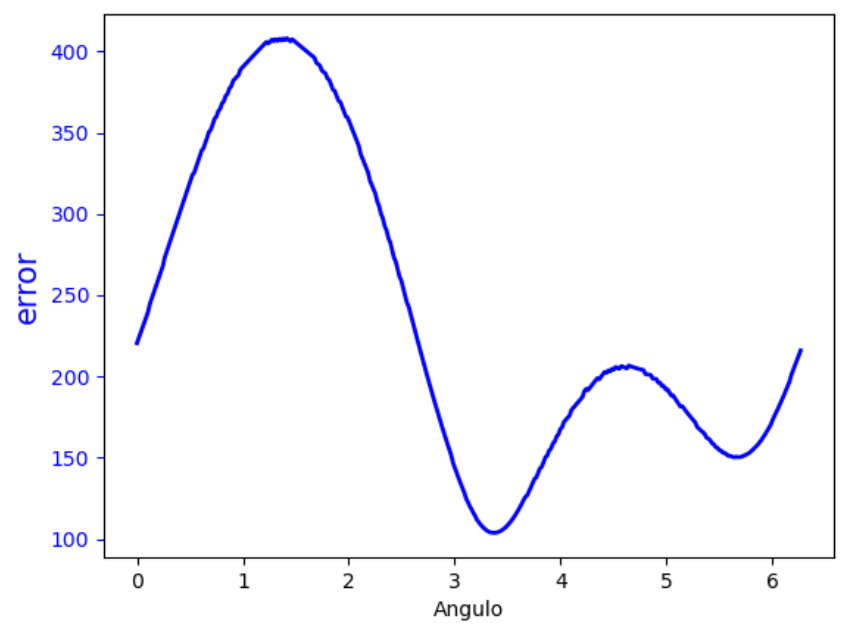
\includegraphics[width=0.5\textwidth]{fotos/gráficas/pregunta2.png}
            \end{wrapfigure}
            
            \vspace{0.1cm}\noindent Para realizar esta cuestión, hemos de modificar el valor del ángulo plano en el programa. Obtenemos así una gráfica que relaciona el error del tiro con el ángulo como vemos en la figura.\\
            
            \noindent Si nos fijamos en la gráfica vemos que esta se minimiza cuando el ángulo es $\pi$ rad (dirección este), cuando la fuerza de Coriolis se minimiza y con ella el error. Volvemos a corroborar que la fuerza de Coriolis es más relevante.\\

        \vspace{-0.4cm}
        \laputa{Utilizando el programa anterior, prueba a modificar la latitud y analiza cómo afecta. Si nos desplazamos al hemisferio Sur (latitudes negativas) se observa algún cambio en las curvas.}

            \noindent Vamos a graficar la trayectoria del tiro puro para distintas latitudes, tanto positivas como negativas.
            
            \begin{figure}[h]
                \centering                
                \begin{subfigure}[t]{.49\textwidth}
                    \centering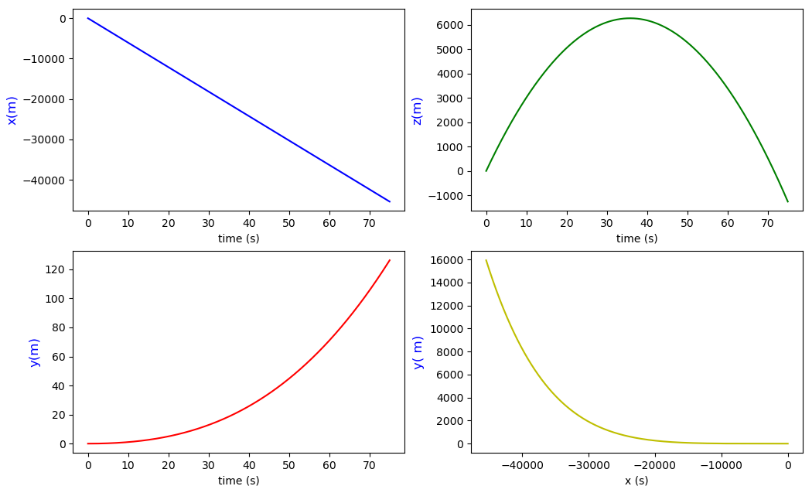
\includegraphics[width=\textwidth]{fotos/gráficas/40.png}
                    \caption{Latitud $40^\circ$}
                \end{subfigure}
                \begin{subfigure}[t]{.485\textwidth}
                    \centering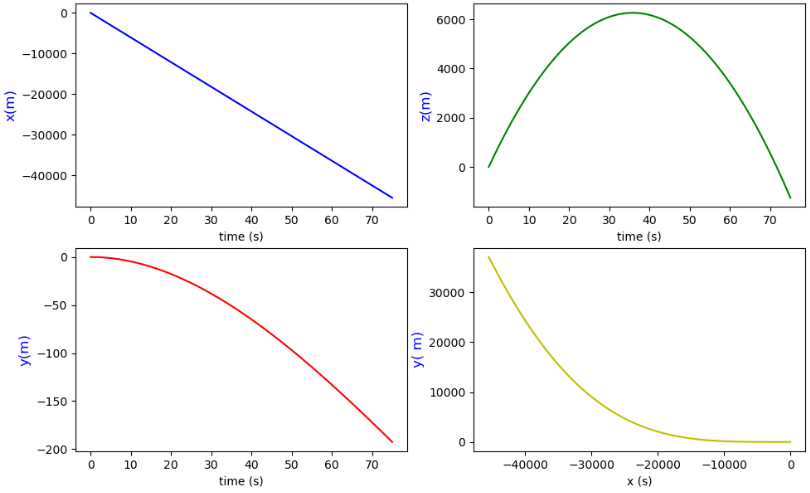
\includegraphics[width=\textwidth]{fotos/gráficas/-40.png}
                    \caption{Latitud $-40^\circ$}
                \end{subfigure}
    
                \begin{subfigure}[t]{.475\textwidth}
                    \centering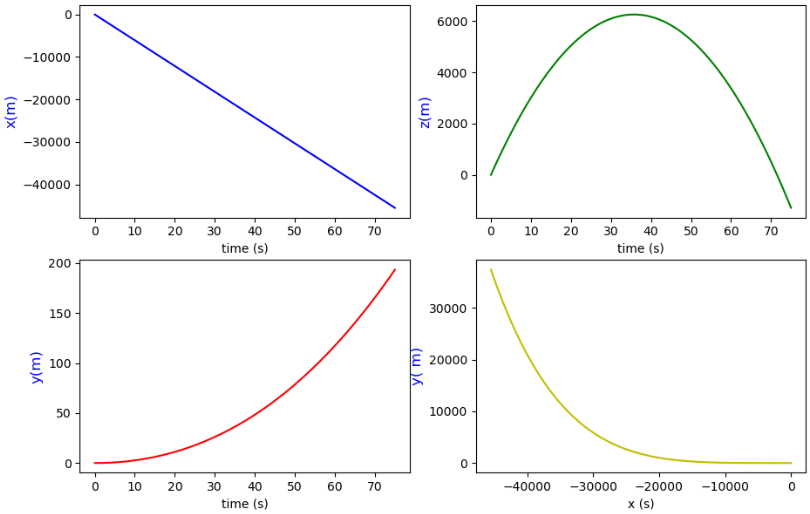
\includegraphics[width=\textwidth]{fotos/gráficas/120.png}
                    \caption{Latitud $120^\circ$}
                \end{subfigure}
                \begin{subfigure}[t]{.495\textwidth}
                    \centering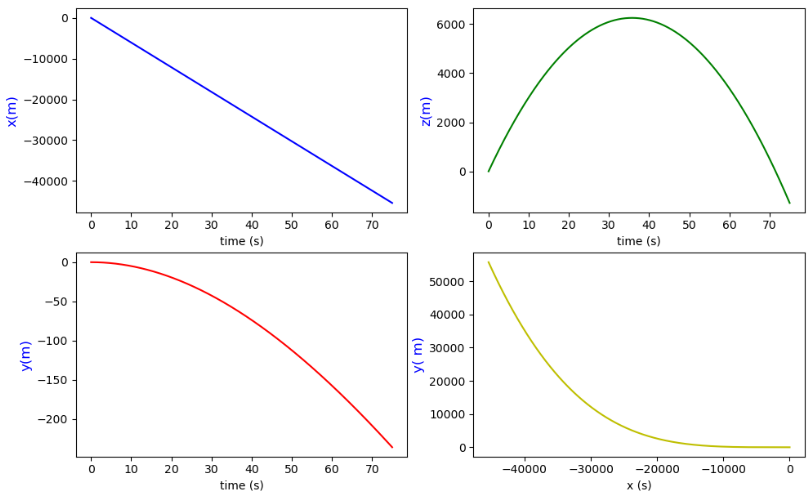
\includegraphics[width=\textwidth]{fotos/gráficas/-120.png}
                    \caption{Latitud $-120^\circ$}
                \end{subfigure}
            \end{figure}

            \vspace{-0.2cm}
            \noindent En las figuras apreciamos como cuando la latitud es positiva (apuntamos hacia el norte) la trayectoria se curva hacia la derecha, mientras que cuando la latitud es negativa (apuntamos hacia el sur) la trayectoria se curva hacia la izquierda. La explicación que tiene este fenómeno es la rotación terrestre, y es que La Tierra gira de Oeste a Este, lo cual explica este cambio en función del signo de la latitud.\\
            \vspace{-0.2cm}
            \begin{wrapfigure}[12]{l}{0.51\textwidth}
                \vspace{-0.6cm}
                \centering
                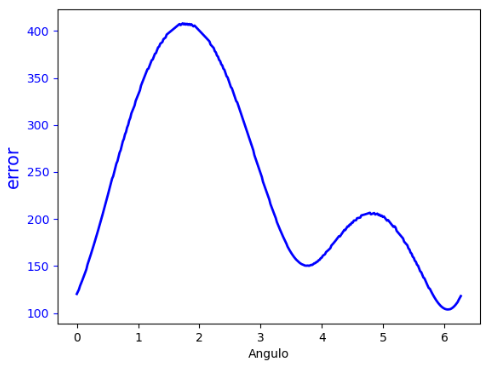
\includegraphics[width=0.5\textwidth]{fotos/gráficas/error-40.png}
            \end{wrapfigure}
            \noindent Ahora vamos a estudiar la función del error para latitudes negativas graficando. Si nos fijamos en los mínimos, ahora los encontramos en $0$ y $2\pi$, es decir, cuando el coseno es 1 y el seno es 0 y se reduce por tanto la aceleración de Coriolis.\\
            
            \vspace{-0.1cm}\noindent Por tanto, concluimos que cuando las latitudes son positivas, el menor error se consigue tirando de Norte a Sur, y cuando las latitudes son negativas, de Sur a Norte.
        
        \clearpage
        \laputa{Con el programa tiro30.py vamos a intentar emular a los artilleros de hace un siglo encontrando una solución de tiro: Entrando un valor concreto de ángulos definimos un tiro parabólico puro. Suponiendo que el punto de impacto es nuestro blanco, utilizando las variables correalz y correpla modifica los ángulos de lanzamiento para que el tiro real caiga lo más cerca posible de la posición predicha por el tiro parabólico. Para ser más realistas, se ha introducido el rozamiento 4 . Si se decide no anular el rozamiento, se recomienda no dar valores superiores a unos 20º al ángulo de alzamiento.}

            \begin{wrapfigure}[12]{l}{0.52\textwidth}
                \vspace{-0.3cm}
                \centering
                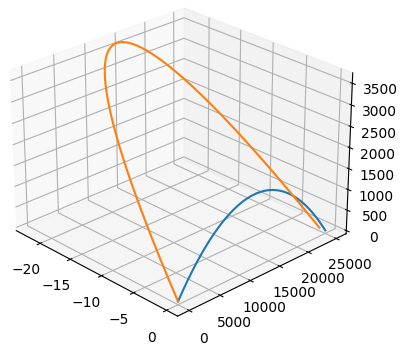
\includegraphics[width=0.5\textwidth]{fotos/gráficas/parabolico.png}
            \end{wrapfigure}
            
            \hspace{0cm}\\\noindent En este apartado, vamos a simular una artillería. Primero calcularemos un tiro parabólico puro (marcado en azul en la figura) y luego calcularemos el tiro real teniendo en cuenta la rotación y el rozamiento.
            
            \begin{itemize}
                \item Tiempo de simulación: $tf=125$
                \item Velocidad de disparo: $velin=700$
                \item Rozamiento: $rz=0.000023$
                \item Latitud: $40$
                \item Ángulo de alzada: $alz=15$
                \item Ángulo sobre el plano: $pla=90$
            \end{itemize}
    
            \noindent Nuestro objetivo era el de minimizar el error entre estos dos tiros. Para ello modificamos las variables \textit{correalz} y \textit{correpla}, a las cuales les haremos un cambio de variable para poder introducir grados en vez de radianes.
            \[correalz = angcorrealz*np.pi/180.0\]
            \[correpla = angcorrepla*np.pi/180.0\]
            
            \noindent Hacemos un proceso de minimización en mi caso graficando el error como función de dos variables, correalz y correpla, y buscando cuando este se minimizaba. Los valores obtenidos son de $\textit{angcorrealz} =10.76^\circ$ y 
            $\textit{angcorrepla} =0.18^\circ$, obteniendo un error en el tiro de $0.87$m. Notar que hay más combinaciones de ángulos que minimizan este error, lo cual podría resultar útil en caso de que una pareja de ángulos fuera demasiado preciso para ser utilizado en algún instrumento real.
            
    \section{Anexos}
        \subsubsection*{Código de LaTeX que genera este documento:}
            \href{https://www.overleaf.com/read/qtqqfwwfdtwq#e56287}{MECN-Practica1:tiro.tex}

\end{document} 